\section{Benchmarking}
\label{sec:benchmarking}

To evaluate our system we compared it with the vendor provided methods
mentioned in section \ref{sec:data_communication}. Timing analysis of
addition and multiplication of varying sized matrices was performed
(two common benchmarks also used in related work
\cite{Rossbach_SOSP11}). Since our focus is on data access and
communication (not computation) we chose matrix addition as a benchmark as it is a
straightforward operation for a GPU to perform. Matrix multiplication
is also included to briefly illustrate how increasing computational
complexity and data accesses affect time to completion. Effective host read and write throughput for each method was also analyzed.

\subsection{Matrix Operations}
Figure \ref{fig:madd_time_spent} shows where the system spends its time in performing a 2048x2048 integer matrix addition using each of the four methods. The time categories are as follows:

\begin{itemize}
 \item {\bf Init: }GPU initialization time.
 \item {\bf MemAlloc: }Memory allocation time (host and/or GPU).
 \item {\bf DataInit: }Time to initialize the matrices.
 \item {\bf HtoD: }Copy time from host to device (\hd).
 \item {\bf Exec: }Execution time of the kernel function.
 \item {\bf DtoH: }Copy time from device to host (\hd\ and \dmh).
 \item {\bf DataRead: }Time to read the result.
 \item {\bf Close: }Free memory and close GPU.
\end{itemize}

\begin{figure}[tb]
\centering
\includegraphics[width=0.5\textwidth, trim=0.0in 3.25in 0.0in 0.25in, clip=true]{eps/madd_time_spent.eps}
\caption{Matrix addition}
\label{fig:madd_time_spent}
\end{figure}
\begin{figure}[tb]
\centering
\includegraphics[width=0.5\textwidth, trim=0.0in 3.0in 0.0in 0.5in, clip=true]{eps/mmul_time_spent.eps}
\caption{Matrix multiplication}
\label{fig:mmul_time_spent}
\end{figure}

First, looking at figure \ref{fig:madd_time_spent} it is clear that using our
\dmh\ method the total time to completion is less than the
others ($34\%$ less than its nearest competitor, \hd). More interesting is the
comparison of how much time is spent for each sub-task. 

For most time categories \dmh\ seems to enjoy the best of each of the
other three: The memory allocation time for \dmh\ is nearly identical to that of
\hd\ and \dm\ and clearly less than \hp. The same is true for the
execution times. Similarly, for data initialization, \dmh\ is just as good
as \hp\ and \dm\ which are superior to \hd. 

\begin{figure}[tb]
\centering
\includegraphics[width=0.45\textwidth, trim=0.0in 2.0in -0.3in 0.74in, clip=true]{eps/madd_time.eps}
\caption{Total Matrix Addition Times}
\label{fig:madd_time}
\end{figure}
\begin{figure}[tb]
\centering
\includegraphics[width=0.45\textwidth, trim=0.0in 2.0in -0.3in 0.72in, clip=true]{eps/mmul_time.eps}
\caption{Total Matrix Multiplication Times}
\label{fig:mmul_time}
\end{figure}

\begin{figure}[t]
\centering
\includegraphics[width=0.45\textwidth, trim=0.0in 2.75in -0.1in 0.60in, clip=true]{eps/write_tput.eps}
\caption{Host Write Throughput}
\label{fig:write_tput}
\end{figure}
\begin{figure}[tb]
\centering
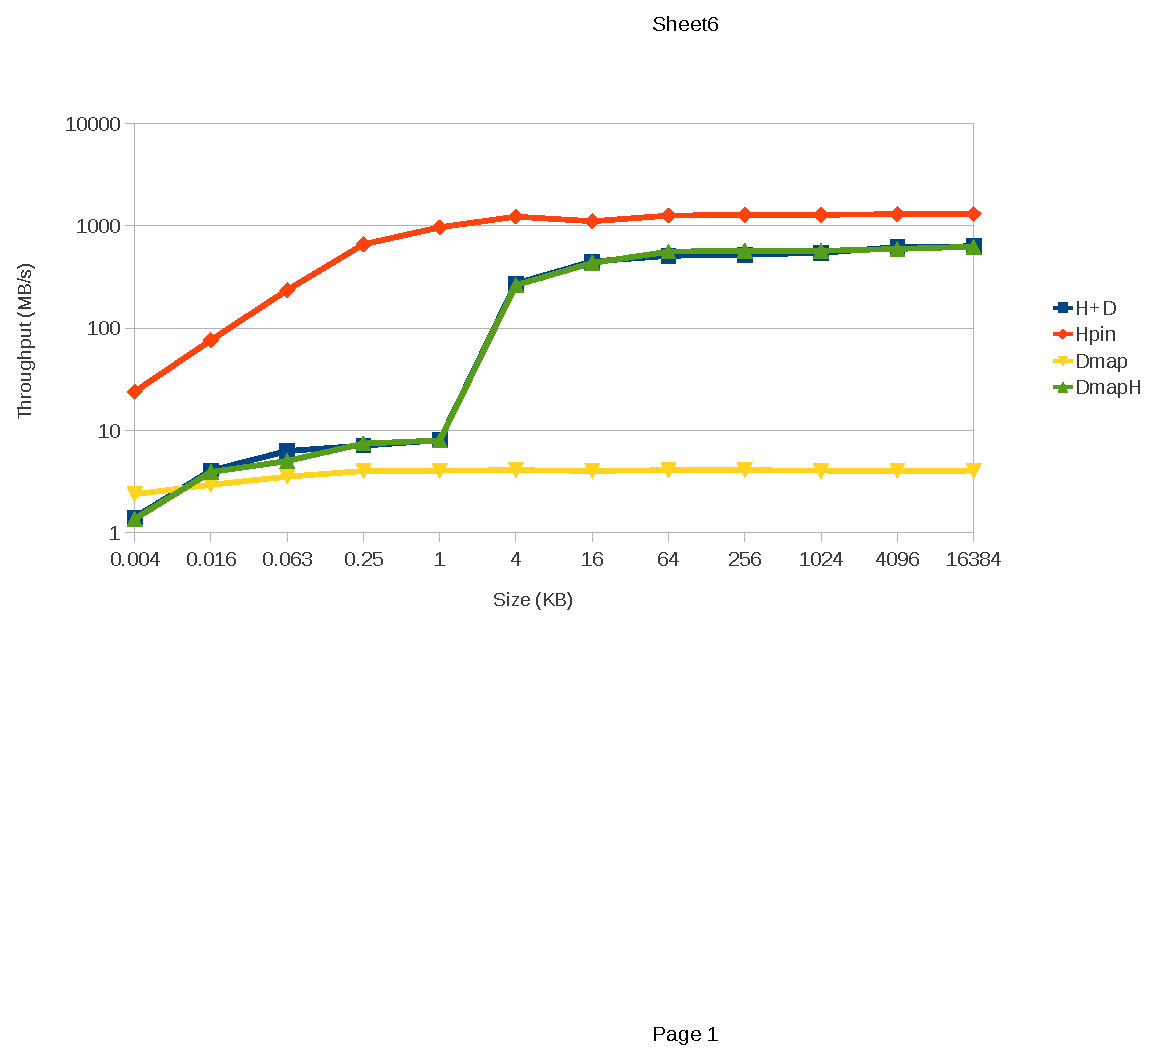
\includegraphics[width=0.45\textwidth, trim=0.0in 2.5in -0.1in 0.6in, clip=true]{eps/read_tput.eps}
\caption{Host Read Throughput}
\label{fig:read_tput}
\end{figure}

The most notable difference among the four methods is the data read time for \dm\ which is orders of magnitude greater than the rest. This represents 16MB of data, read 4 bytes at a time across the system buses and is the motivation for our \dmh\ method. Instead of reading one matrix element at a time, \dmh\ first copies the data to the host before reading.

The same anomaly is present in the execution time for \hp\ -- the GPU must read one element at a time from the host memory (in the other three methods the data reside on the GPU during computation). This makes \hp\ increasingly inferior as data sizes grow.

Figure \ref{fig:mmul_time_spent} shows the same time analysis for matrix multiplication. The only difference occurs in the execution times. This is not surprising as the multiplication experiments are exactly the same as addition with the exception of the kernel function on the GPU. In fact, if execution times were omitted, figures \ref{fig:madd_time_spent} and \ref{fig:mmul_time_spent} would look identical.

%One thing to note, however, is the amount by which the execution times have increased. For each element in the output matrix, there will be $2n$ data reads, $n$ multiplications, and $1$ data write where $n$ is the length and width of the matrices (as opposed to $2$ accesses, $1$ addition and $1$ write).   

While this does present a real-world scenario, in a real-time system it is
more likely that tasks will be performed repeatedly and therefore
the GPU initialization and closing costs might occur only once -- the
same context with kernel function(s) loaded would remain active while
only the data might change. Furthermore, it could be the case that the
memory allocated for the task could be reused and only the contents
modified. For these reasons, the remainder of our analysis focuses only on reads, writes, transfers, and execution. 

Figure \ref{fig:madd_time} shows the time to completion of matrix
addition as a function of matrix size (note the logarithmic
scale). \hp\ appears to be the best performer until a matrix size of
$32\times32$ (corresponding to a data size of 4KB for each matrix) at
which point \dmh\ becomes superior. This is also reflected in the
matrix multiplication times (figure \ref{fig:mmul_time}). One thing to
note is the growth rate of \hp\ in matrix multiplication; Since each
thread must perform multiplication and addition $n^2$ times (compared
with one addition in matrix addition), the number of reads that occur
across the buses increases by a greater exponential factor. We expect that the time for \hp\ would eventually surpass \dm\ as the trend in the graph indicates.


%Note that even with the logarithmic time scale the curves appear exponential because while the matrix length and width increase as $2^n$ the data size of the
%matrix is $2^n \times 2^n \times 4 =  2^{2n+2}$ bytes (for 32-bit integers).


\subsection{Data Throughput}
Figure \ref{fig:write_tput} shows the effective host write throughput
as a function of data size.  We use the term `effective throughput' to
mean ($size/time$) where $time$ is measured from the beginning of data
initialization to the point at which it is actually available to
the GPU. For example, in the case of \hd\, this corresponds to the total time for the host to write to each element in the data structure (which
is in main memory) plus the time to copy the data to the GPU.

Figure \ref{fig:write_tput} shows that the write throughput of \dmh\
is better than \hd\ by about a factor of 2 and at least as good as the others (\hp, \dm, and \dmh\ all coincide
almost exactly in the graph). Figure \ref{fig:read_tput} paints a
slightly different picture for read throughput. It should not be
surprising that \hp\ outperforms the rest as it represents the host
iterating over a data structure that is already in host memory. \hd\
and \dmh, on the other hand, must first copy the data from the GPU to
the host and they achieve roughly equal performance (they coincide in
the graph). Finally, \dm\ is
the weakest performer because of the large number of small reads that
occur across system buses (as explained earlier).
